\documentclass[tikz,border=3.14mm]{standalone}
\usepackage{pgfplots}
\pgfplotsset{compat=1.18}

\begin{document}
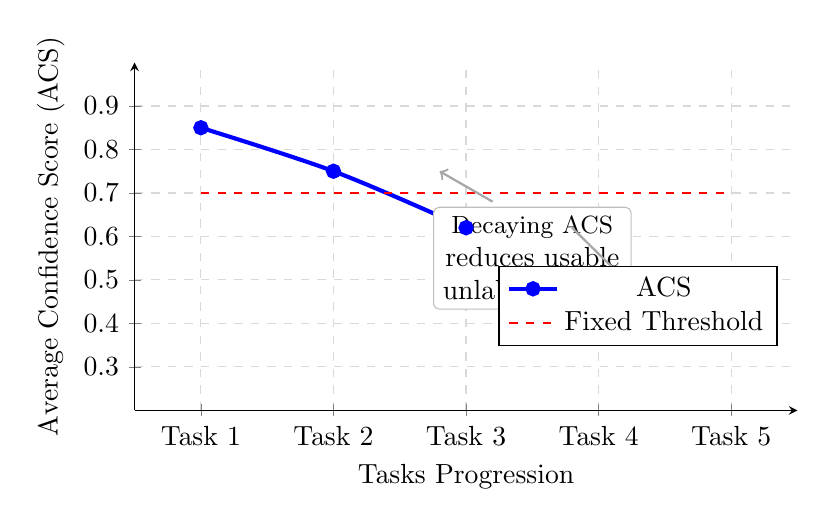
\begin{tikzpicture}
\begin{axis}[
    xlabel={Tasks Progression},
    ylabel={Average Confidence Score (ACS)},
    xmin=0.5, xmax=5.5,
    ymin=0.2, ymax=1.0,
    xtick={1,2,3,4,5},
    xticklabels={Task 1, Task 2, Task 3, Task 4, Task 5},
    ytick={0.3,0.4,0.5,0.6,0.7,0.8,0.9},
    grid=both,
    grid style={dashed, gray!30},
    axis lines=left,
    width=10cm,
    height=6cm,
    legend style={at={(0.97,0.3)}, anchor=east}
]

% ACS Decay Curve
\addplot[
    color=blue,
    mark=*,
    line width=1.5pt,
    smooth
] coordinates {
    (1,0.85)
    (2,0.75)
    (3,0.62)
    (4,0.48)
    (5,0.38)
};
\addlegendentry{ACS}

% Fixed Threshold Line
\addplot[
    color=red,
    dashed,
    line width=1pt
] coordinates {
    (1,0.7)
    (5,0.7)
};
\addlegendentry{Fixed Threshold}

% Annotations
\node[align=center, fill=white, rounded corners=2pt, draw=gray!50] 
    at (3.5,0.55) {\small Decaying ACS\\reduces usable\\unlabeled data};

\draw[->, thick, gray!70] (3.2,0.68) -- (2.8,0.75);
\draw[->, thick, gray!70] (3.8,0.62) -- (4.2,0.5);

\end{axis}
\end{tikzpicture}
\end{document}